\documentclass[border=0.8ex,svgnames,tikz]{standalone}
\usepackage{amsmath,mathtools}
\usepackage{fontspec}
\setmainfont{Source Serif 4}
\setsansfont{Source Sans 3}
\setmonofont{Source Code Pro}
\usetikzlibrary{positioning,calc}
\def\xcoloruseA{MediumBlue}
\def\xcoloruseB{LimeGreen}
\def\xcoloruseC{Crimson}
\begin{document}
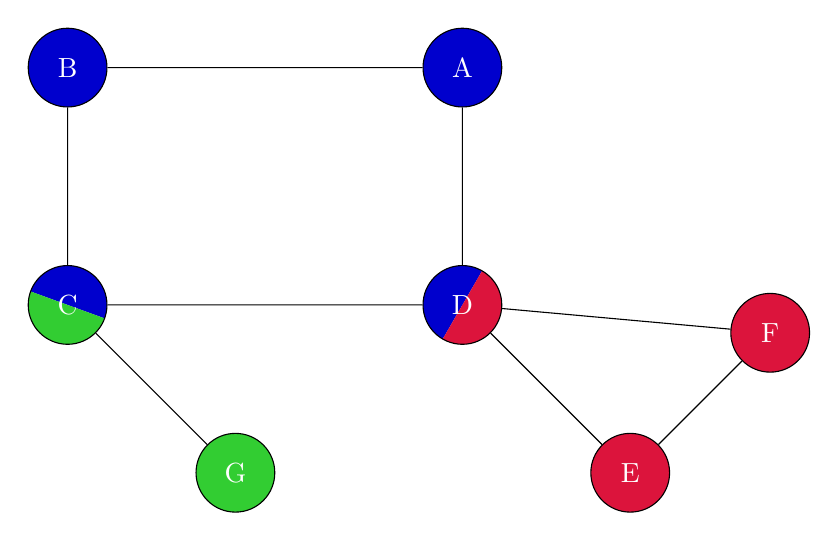
\begin{tikzpicture}[
  node split radius/.initial=1,
  node split color 1/.initial=red,
  node split color 2/.initial=green,
  node split color 3/.initial=blue,
  node split half/.style={node split={#1,#1+180}},
  node split/.style args={#1,#2}{
    path picture={
      \tikzset{
        x=($(path picture bounding box.east)-(path picture bounding box.center)$),
        y=($(path picture bounding box.north)-(path picture bounding box.center)$),
        radius=\pgfkeysvalueof{/tikz/node split radius}}
      \foreach \ang[count=\iAng, remember=\ang as \prevAng (initially #1)] in {#2,360+#1}
      \fill[line join=round, draw=none, fill=\pgfkeysvalueof{/tikz/node split color \iAng}]
      (path picture bounding box.center)
      --++(\prevAng:\pgfkeysvalueof{/tikz/node split radius})
      arc[start angle=\prevAng, end angle=\ang] --cycle;
    },
  },
  every node/.style={draw,circle,minimum size=1cm,text=White},
  every path/.style={draw,>=latex},
  x1color/.style args={#1}{fill=#1},
  x2color/.style args={#1|#2|#3}{node split color 1=#1,node split color
    2=#2,node split half=#3},
  ]
  \coordinate(graph);
  \node[x1color={\xcoloruseA},below=of graph] (Agraph) {A};
  \node[x1color={\xcoloruseA},left=4cm of Agraph] (Bgraph) {B};
  \node[x2color={\xcoloruseA|\xcoloruseB|-20},below=2cm of Bgraph] (Cgraph) {C};
  \node[x1color={\xcoloruseB},below right=2.0cm of Cgraph] (Ggraph) {G};
  \node[x2color={\xcoloruseA|\xcoloruseC|60},below=2.0cm of Agraph] (Dgraph) {D};
  \node[x1color={\xcoloruseC},below right=2.0cm of Dgraph] (Egraph) {E};
  \node[x1color={\xcoloruseC},above right=1.5cm of Egraph] (Fgraph) {F};
  \path
  (Agraph) -- (Bgraph) -- (Cgraph) -- (Dgraph) -- (Agraph)
  (Cgraph) -- (Ggraph)
  (Dgraph) -- (Egraph) -- (Fgraph) -- (Dgraph);
\end{tikzpicture}
\end{document}
